\chapter{Code Dokumentation mit Doxygen}

\section{Dokumentation \& Code-Dokumentation}

\subsection{Zweck der Dokumentation}

\begin{itemize}
	\item  Wissenssicherung: \\ Wissen über ein System macht einen beträchtlichen Wert des Systems aus --> Menschen vergessen schnell
	\item Förderung der Kommunikation \& Genauigkeit 
	\item Sichtbarmachen des  Projektfortschrittes: \\ Fertigstellung und Freigabe von Dokumenten markiert nachprüfbar(!) den Projektfortschritt
\end{itemize}

Bei der Programm-Dokumentation werden bestehende Programmteile (v.a. Schnittstellenbeschreibungen (APIs)) verwendet. Der Entwickler / Programmierer dokumentiert, wenn das bestehende Programm verändert wird.

Die Dokumentation im Code hat den Vorteil, dass Dokumentationen bei Änderungen häufig nicht nachgeführt wurden, da Code und Dokumentation getrennt waren. Dies führte zu Inkonsistenzen sowie fehlerhaften und unvollständigen Dokumentationen.

Code-Dokumentationen integrieren Beschreibungen in den Source-Code mit Hilfe von speziellen
Kommentaren. Die Dokumentation wird erzeugt mit Hilfe von Dokumentationswerkzeugen, die den Sourcecode analysieren und die Beschreibung daraus extrahieren.

\subsection{Vorteile von Code-Dokumentation}
\begin{itemize}
	\item Erzeugung der Dokumentation kann leicht automatisiert werden. --> Dokumentation bleibt aktuell
	\item Gewisse Informationen, wie z.B. Funktionsköpfe, werden direkt aus dem Programmcode 
	entnommen.  
	\item Dadurch, dass Beschreibungen und Source-Code unmittelbar nebeneinander im Source-Code-
	Dokument vorkommen, ist die Wahrscheinlichkeit gross, dass Programmcode und Beschreibung 
	übereinstimmen. --> Dokumentation bleibt konsistent
	\item Vor allem geeignet zur API-Dokumentation von Klassen bei der Objektorientierten 
	Programmierung.
	\item Hinweis auf gewisse nicht dokumentierte Codestellen (z.B. Parameter) leichter. --> Dokumentation ist vollständig
\end{itemize}

\section{Doxygen}
- The KDE API Reference (Linux Desktop): http://api.kde.org/ \\
- D-Bus documentation (SW Message Bus System): http://freedesktop.org/software/dbus/doc/api/html/index.html \\
- The Xerces-C++ Documentation (XML-Parser): http://xerces.apache.org/xerces-c/apiDocs-3/classes.html \\

Weit verbreitetes Dokumentationswerkzeug:  \\
- Open Source, für Windows, Unix / Linux, Mac, … \\
- unterstützt: C, C++, Java, C\#, etc. \\

Erzeugt Dokumente in folgenden Formaten: \\
- HTML (für Browser) – am häufigsten \\
- LaTeX (dvi, pdf mit Links, PostScript …) \\
- Unix man pages \\
- RTF (MS-Word) \\
- XML (für maschinelle Weiterverarbeitung) \\
Erstellt primär API-Beschreibungen, aber (mit Zusätzen) auch Klassendiagramme und andere 
Diagramme. \\
Weitere Infos, Website:  http://www.stack.nl/~dimitri/doxygen/

\begin{figure}[ht]
	\centering
	\adjustbox{width=11cm}{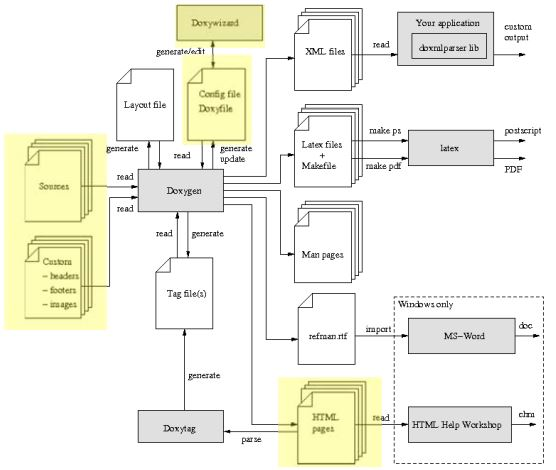
\includegraphics{Figures/darchitektur}}
	\caption[]{Doxygen Architektur}
\end{figure}

Doxygen ist ein "Command-Line-Tool". \\
GUI-Frontend "doxywizard" sowie Plugins z.B. für Eclipse («Eclox») \\
Hauptbefehl (command-line): \$ doxygen \\
Doxygen benötigt eine Konfigurationsdatei: "Doxyfile" \\
Aktuelle Anzahl möglicher Konfigurationen: 267 \\ 
Aufruf-Beispiele: \\
\$ doxygen -g     // erzeugt Konfigurationsdatei "Doxyfile" \\
\$ doxygen Doxyfile // erzeugt Dokumentation, falls Konfig'datei Doxyfile heisst, reicht:\$ doxygen

\subsection{Wichtigste Einstellungen}
- Projektname: PROJECT\_NAME = "Voltage Divider" \\
- Input: INPUT = . ./src ./tests README.md \\
- Datei-Filter: FILE\_PATTERNS = *.cpp, *.h \\
- Output: OUTPUT\_DIRECTORY = doc \\
- README.md als mainpage: USE\_MDFILE\_AS\_MAINPAGE = README.md \\

\subsection{Wichtigste Befehle für Doxygen}
Allgemein \\
- Dateikopf \\
- file \\
- date \\
- author \\

Funktionsbeschreibung \\
- brief \\
- param \\
- pre \\
- post \\

Beispiel: \\
/// \textbackslash brief Calculates the optimal values for R1 and R2. The base formula \\
///        behind this calculation is \textbackslash f$u1=u2 {r2 \over r2+r1}\textbackslash f$. \\
/// \textbackslash pre \textbackslash p u1 > \textbackslash p u2 \\
/// \textbackslash pre \textbackslash p lowerRTh < \textbackslash p upperRTh \\
/// \textbackslash param u1 Value for U1 in V \\
/// \textbackslash param u2 Value for U2 in V \\
/// \textbackslash param lowerRTh set the lower bound for resistor value output \\
/// \textbackslash param upperRTh set the higher bound for resistor value output \\
/// \textbackslash param resDecade gives the resister e-decade on which the resistor are calculated  
virtual void calc(double u1, double u2, double lowerRTh, double upperRTh,
const EDecade\& resDecade); \\

\begin{figure}[ht]
	\centering
	\adjustbox{width=10cm}{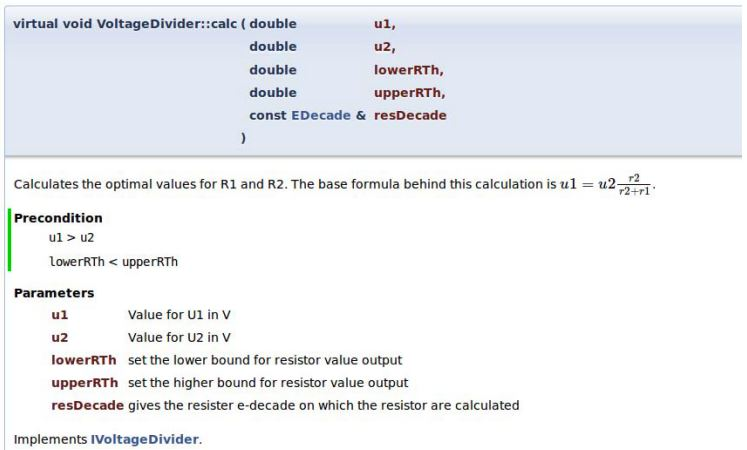
\includegraphics{Figures/dhtmlausschnitt}}
	\caption[]{Ausschnitt aus dem HTML-Output}
\end{figure}


Die Doxygen Hauptseite wird als erstes in der HTML Dokumentation angezeigt. \\
Zweck: Sie soll einen Überblick über das gesamte Projekt vermitteln \\
Formatierungsanweisung:  @mainpage oder markdown file (z.B. README.md, empfohlen)

\subsection{Weitere Informationen zu Doxygen}
Ein Markdown-File (typischerweise README.md genannt) enthält eine Plain Text Formatierungssyntax. Das Ziel ist dabei es so leserlich wie möglich zu machen. Es soll als plain Text publiziert werden wie es ist, ohne visueller Überladung durch zusätzliche Syntax. \\
Beispiel: \# This is an H1 Header \# oder \#\# This is an H2 Header \#\# \\
Es kann kann mit folgendem Befehl verwendet werden: USE\_MDFILE\_AS\_MAINPAGE = README.md \\
INPUT = ./tests ./src README.md  \\
Die erste Zeile wird im Titelbalken dargestellt. Mit einem Punkt wird der Projektname verwendet. Der Nachteil bei dieser Lösung ist eine Warnung beim Übersetzten \\
Weitere Syntax: http://daringfireball.net/projects/markdown/syntax \\

\subsubsection{Code Documentation Style}

\begin{minipage}{8cm}
 Java / C 
\end{minipage}
\begin{minipage}{3cm}
	C
\end{minipage}
\begin{minipage}{3cm}
	C++
\end{minipage}
\begin{minipage}{3cm}
	C++
\end{minipage}

\adjustbox{width=8cm}{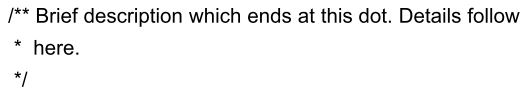
\includegraphics{Figures/textstylejava}}
\adjustbox{width=3cm}{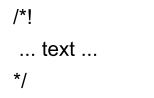
\includegraphics{Figures/textstylec}}
\adjustbox{width=2cm}{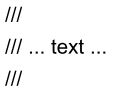
\includegraphics{Figures/textstyle}}
\adjustbox{width=2cm}{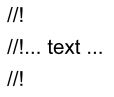
\includegraphics{Figures/textstyle2}}

\textbackslash \textbackslash  sind hier wichtig. Sie schliessen einen normalen Kommentarblock und öffnen einen C-Style Kommentarblock. 

\subsubsection{Weitere Befehle für Doxygen}

Jeder Befehl beginnt mit @ oder \. \textbackslash wird häufig für C/C++ und @cmd oft für Java genutzt. 
LaTex Formeln sind kompatibel für Outputs in LaTeX und HTML. \\
Dabei muss USE\_MATHJAX eingeschaltet sein. \\
Beispiel: \textbackslash f\$formel\textbackslash f\$\\
Bilder sind kompatibel für Outputs in LaTeX, HTML, Docbook und Rtf. \\
Dabei muss IMAGE\_PATH auf den Pfad mit den Bildern zeigen. \\
Beispiel:  \textbackslash image format file "caption" \\
\textbackslash image html Kontextdiagramm.gif "Kontext-Diagramm" \\
\textbackslash image latex Kontextdiagramm.eps "Kontext-Diagramm" width=10cm \\
